\section{Introduction}
\label{sec:intro}

Electromigration is considered the top killer for today's copper dual
damascene interconnect technology. Recently there is a renewed
interests in EM modeling and mitigation techniques as EM induced
reliability is geting worse as technology advance.  ITRS predicts that
the EM induced life time of the interconnects will be reduced by half
by each generation~\cite{ITRS}. To make this situaiton more worse,
many widely used EM models such as Black-Blech models are thought to
be too conservative, which can lead to significant over
designs~\cite{Bailey:semieng}.

Existing EM model and analysis techniques mainly focus on the simple
straight line interconnect with two line end
terminals~\cite{deOrio:2010}.  Exsiting widely used EM models such as
Blech limit \cite{Blech:1976ko} (for the out filtration of immortal
segments) and Black's equation \cite{Black:1969fc} (for calculating
MTTFs for segments characterized by known current densities and
temperatures) are subjects of the hard criticism
\cite{Ohring:1998uj}\cite{Lloyd:2008je}\cite{Hauschildt:2013cv} as
those emperical models are stressing condition dependent and lacks of
scalability over wide current and temperature stressing
conditions. More importantly, those models can only applied to simple
wire strucutres.  For practical VLSI chips, the interconnects such as
clock and power grid networks typically consist of multi-branch metal
segments representing a continuously connected, highly conductive
metal (Cu) lines within one layer of metallization, terminating at
diffusion barriers, which are commonly seen in the power/ground
network in practical VLSI layouts.  The EM effects in those branches
are not independent and they have to be considered simultaneously.  To
further illustrate this, we consider a 4-segment and 5-terminal
interconnect wire loaded with DC voltage distribuation as shown in
Fig.~\ref{fig:4seg-demo}. The finite element analysis (FEA) can be
used to calculate the calculate the current and the resulting
hydrostatic stress along the interconnect wire.  The distributions
of the hydrostatic stress, current density and voltage potential along
this wire are shown in Fig. \ref{fig:4seg-multiplot} (from top to
bottom) respectively. As we can see that although the segment 2 has
almost zero current density, its tensile (positive) stress is the
highest. As a result, we have to analyze all the stress evolution as a
whole instead of treating each segment seperately as done in the
existing EM assessment methods.

\begin{figure}[h]
\centering
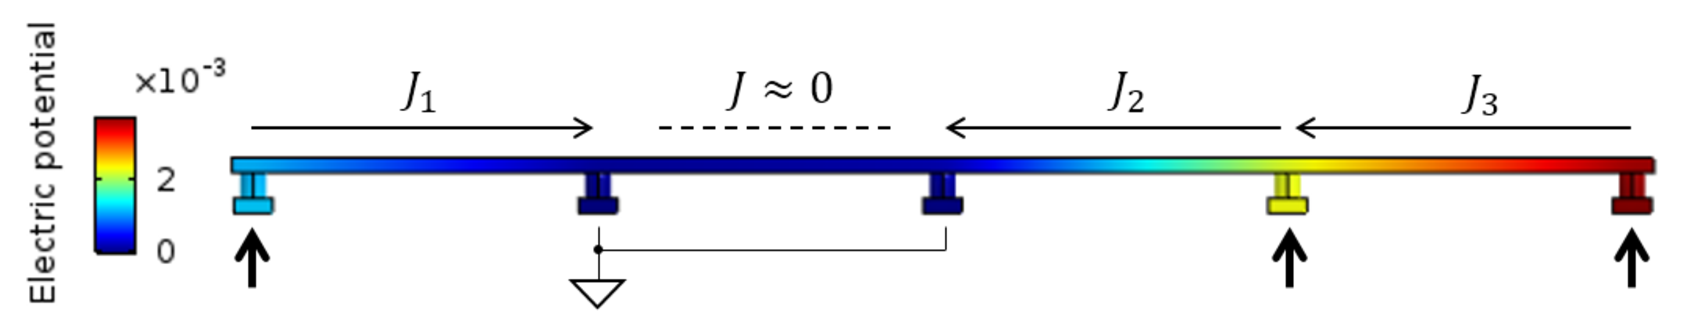
\includegraphics[width=0.95\columnwidth]{4seg_demo}
\caption{Electrical current in a 4-segment wire structure (J: current direction)}
\label{fig:4seg-demo}
\end{figure}

\begin{figure}[h]
\centering
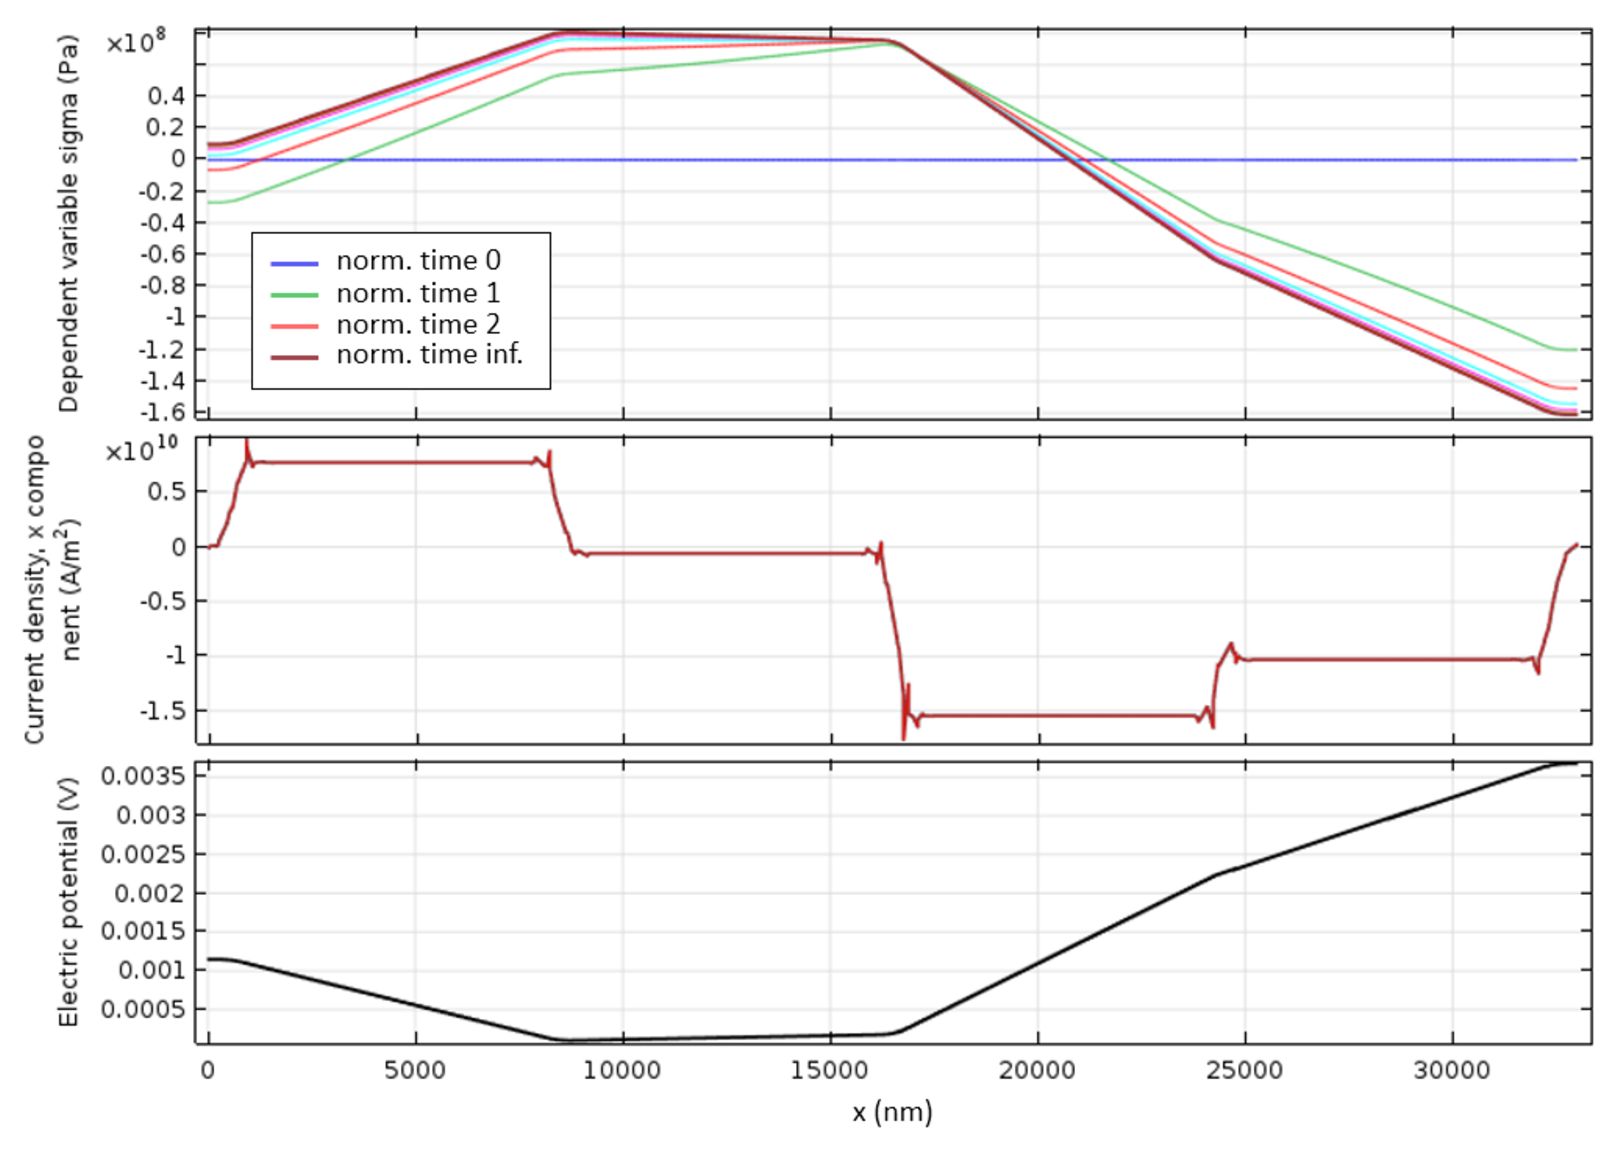
\includegraphics[width=0.95\columnwidth]{4seg_multiplot}
\caption{Hydrostatic stress, current density, and voltage distribution in the 4-segment wire structure}
\label{fig:4seg-multiplot}
\end{figure}


Recently some physics-based EM analysis methods for the
TSV and power grid networks have been proposed based on solving the
basic mass transport
equations~\cite{Pak:2011cx,Pathak:2011kz,Zhao:2013cv,Pak:2013bh}.
Those models treat the resistance changes of a wire over time as the
atomic concentration changes due to atomic flux. Since these proposed
methods solve the basic mass transport equations using the finite
element method, they can only solve for very small structures such as
one TSV structure. Complicated look-up table or models have to be
built for different TSVs and wire segments for full-chip power grid
analysis at reduced accuracy.

To mitigate this problem, a more compact physics-based EM model was
proposed recently in ~\cite{HuangYu:DAC'14}. It is based on the
hydrostatic stress diffusion
equation~\cite{Korhonen:jap1993}. However, this EM model still works
for one single wire segment. Although the new EM model has been
extended to deal with multiple branch tree wire based on projected
steady-state stress.  It still can't provide the time-dependent
hydrostatic evolution of hydrostatic stress, which ultimately
determines the failures for multi-branch interconnect wires.  Recently
EM models for multi-branch interconnect tree have been
proposed~\cite{ChenHuang:DAC'15,ChenTan:TCAD'16}. In this approach,
analytic solutions for stress evolution were derived for a few
specific interconnect structures. Moreover, those those analytic
expressions are still can be applied to more general structures such
as the multi-segment interconnect wires as shown in



% Many researchers have studied the evolution of stress due
% to electromigration. Kirchheim proposed a physically based model in
% which generation of stress in grain boundaries during electrimigration
% is caused by the annihilation and generation of vacancies. Korhonen
% ~\cite{Korhonen:jap1993} proposed another physically based analytical
% model for mechanical stress evolution during electromigration in a
% confined metal line described by a one-dimensional equation, as
% follows:

%\% begin{equation}
% \label{eq:basic_em}
% \frac{\partial \sigma(x,t)}{\partial t}=\frac{\partial }{\partial x}\left[\frac{D_aB\Omega}{kT}\left(\frac{\partial \sigma(x,t)}{\partial x}+\frac{Z^*e\rho}{\Omega}j\right)\right]
% \end{equation}
% where $\sigma$ is the hydrostatic stress, $t$ is time, $D_a$ is the atomic diffusivity, $B$ is the effective bulk modulus, $\Omega$ is atomic volume,$k$ is the Boltzman's constant, $T$ is absolute temperature, $Z^*$ is the effective charge number, $e$ is electron charge, $\rho$ is resistivity, and $j$ is current density. Our works were mainly based on Equation
% \eqref{eq:basic_em}. The advantage of this model is that the evolution of hydrostatic stress in the confined line can be calculated in a closed form, which has been widely used in EM analysis. For the sake of simplicity, we rewrote Equation \eqref{eq:basic_em} as follows:

% \begin{equation}
% \label{eq:basic_em_s}
% \frac{\partial \sigma(x,t)}{\partial t}=\frac{\partial }{\partial x}\left[D_t\left(\frac{\partial \sigma(x,t)}{\partial x}+G\right)\right]
% \end{equation}
% where $D_t=\frac{D_aB\Omega}{kT}$ is the stress diffusivity affected by temperature $T$ and $G=\frac{Z^*e\rho}{\Omega}j$ is EM driving force. Moreover, $D_a=D_0e^{-\frac{E_a}{kT}}$ is the effective atomic diffusion coefficient. $D_0$ and $E_a$ stand for the pre-exponential factor and the activation energy, respectively.

% \begin{figure}[!h]
% \centering
% 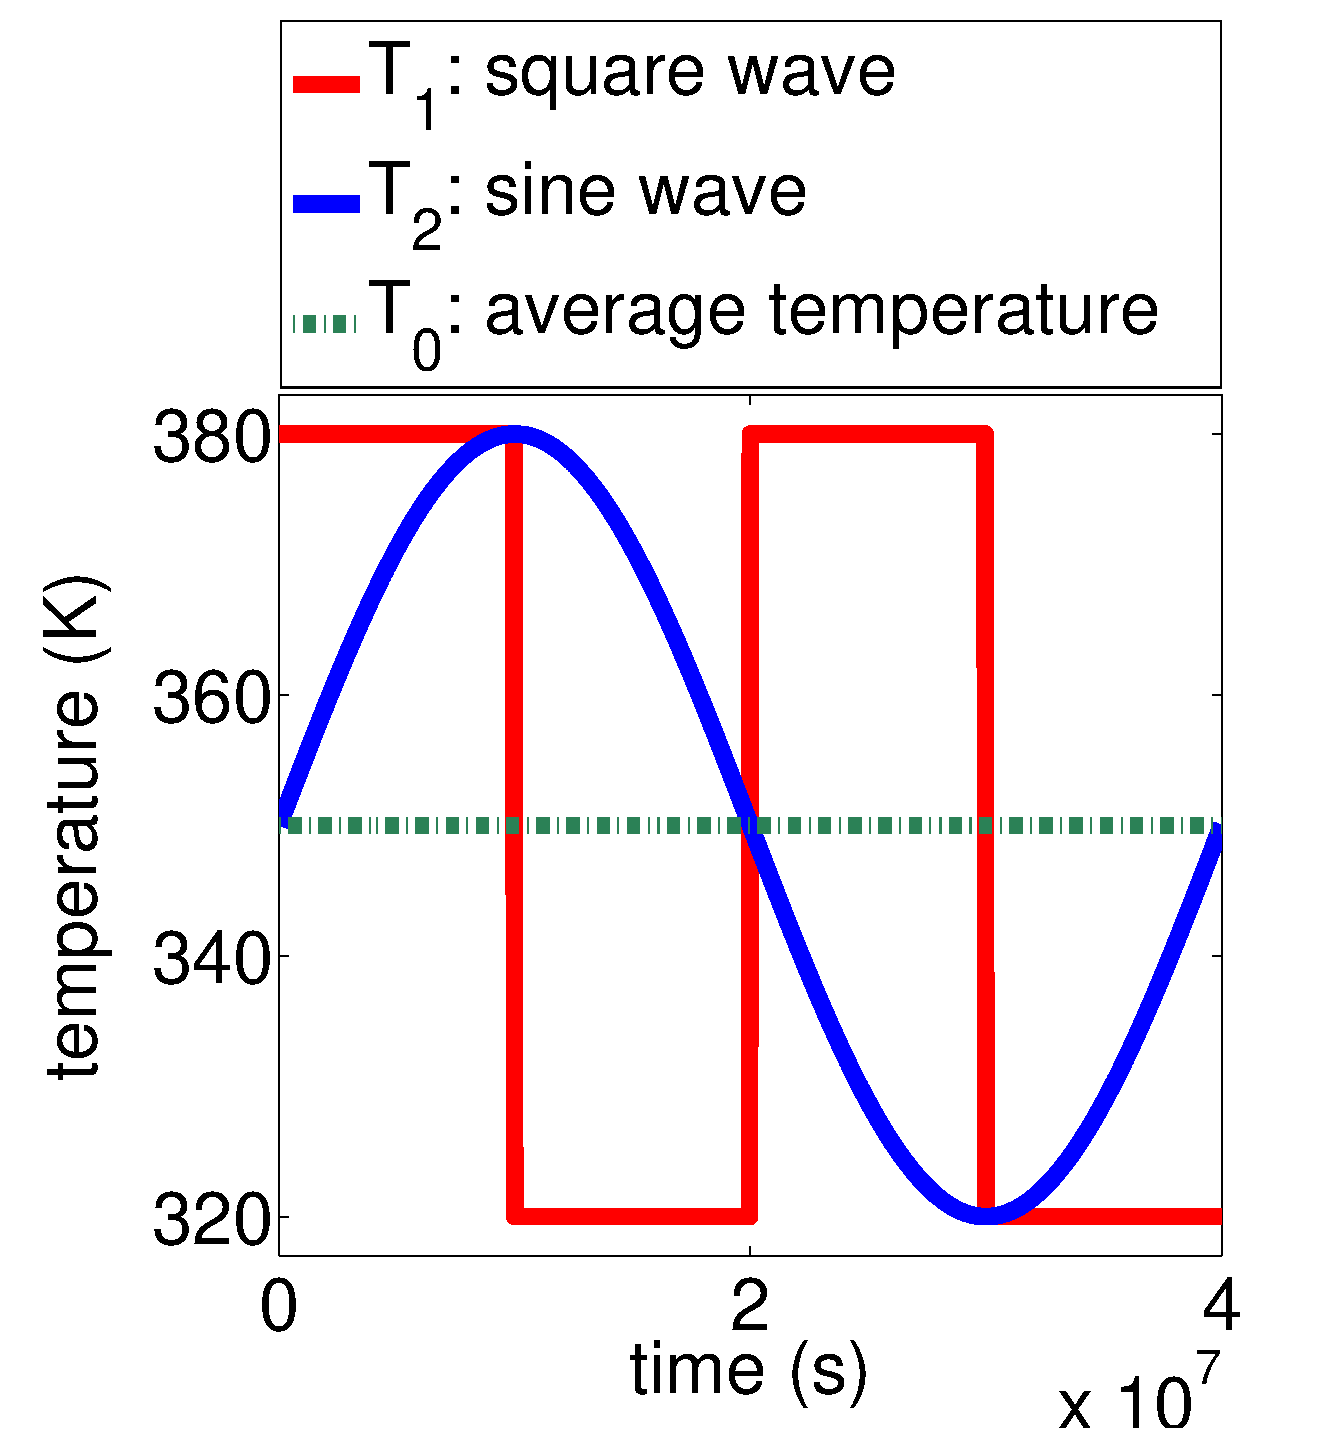
\includegraphics[width=2in]{DifferentTemperature.eps}
% \caption{The different temperature function in later experiments.}
% \label{fig:NTTemperature}
% \end{figure}

% The research for multi-branch interconnect trees is still a large and
% challenging problem. Due to the strong thermal-dependence of leakage
% power, circuit performance, IC package cost and reliability, thermal
% effects has become a recent major research for being a limiting factor
% in high performance circuit design. Among the thermal effects, varying
% temperature is an important part to EM analysis. We have made the EM
% experiments considering the changing temperature and the average
% temperature. In Fig.\ref{fig:NTTemperature}, we create three types of
% changing temperature. As we can see, function $T_0(t)$ is the average
% temperature of square wave temperature $T_1(t)$ and sine wave
% temperature $T_2(t)$. The stress evolution results for straight line
% interconnect tree simulated in COMSOL are showed in
% Fig.\ref{fig:NoteTemperature}, indicating that the relative stress
% variation is mostly higher than 0.5. Explicitly, we can't use average
% temperature to replace the changing temperature.

% \begin{figure}[!h]
% \centering
% \subfigure[]{
% 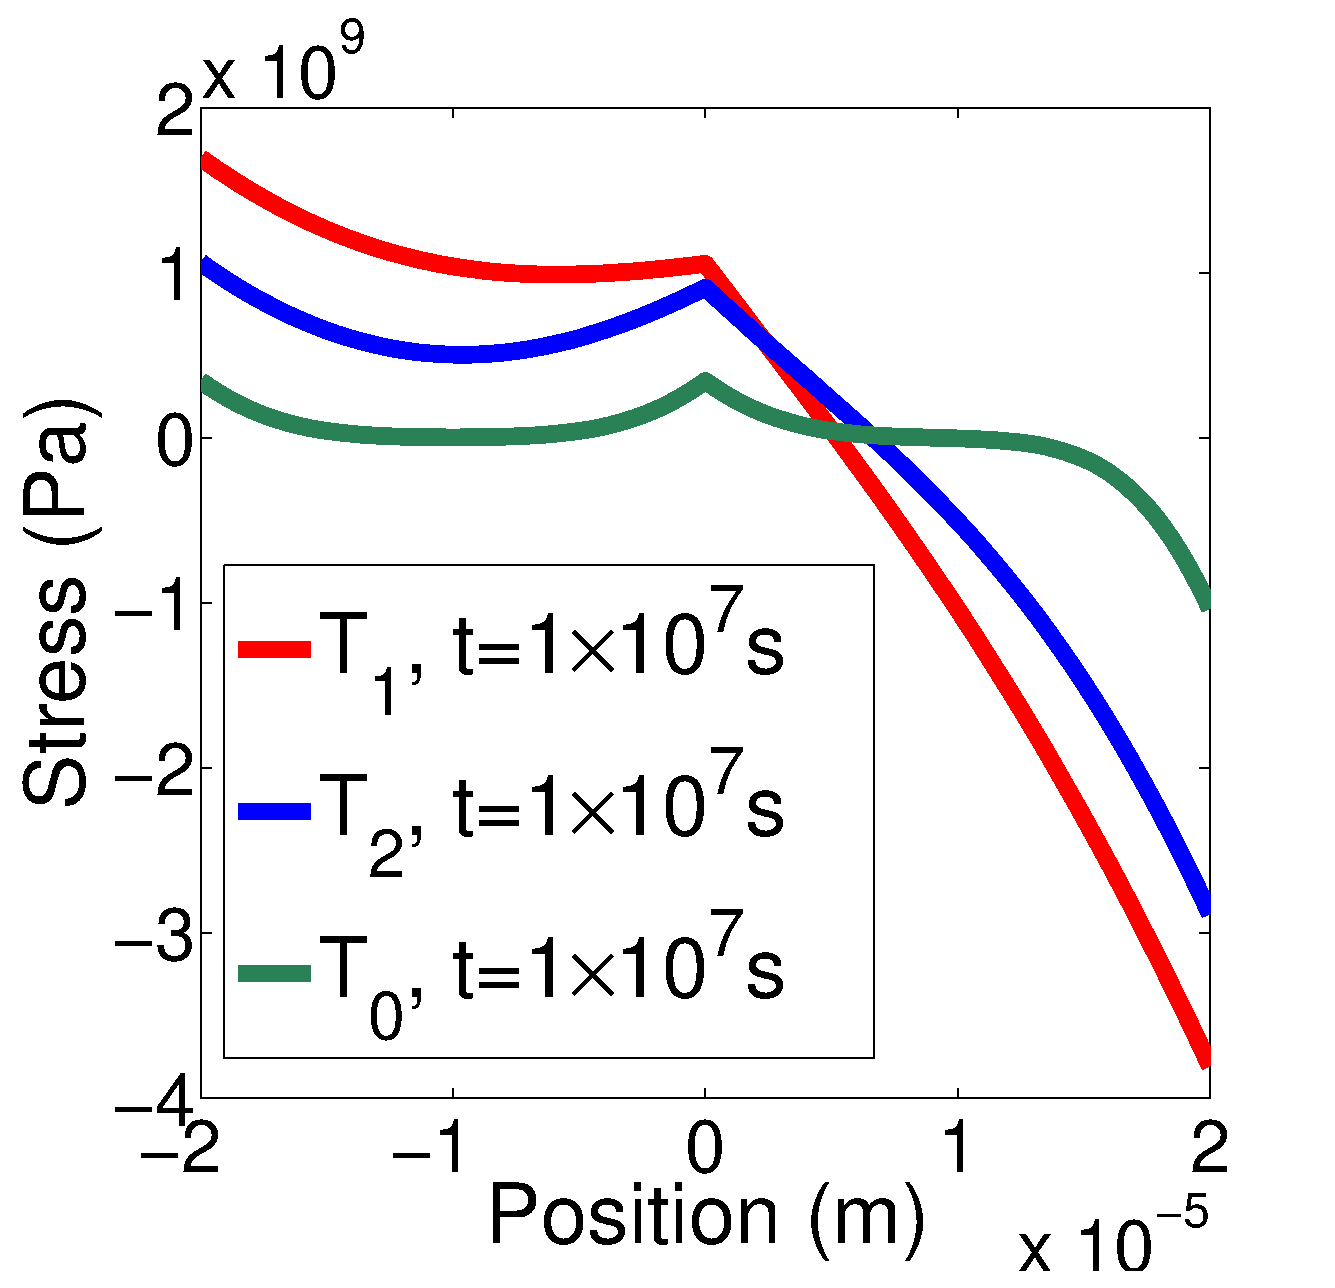
\includegraphics[width=0.45\columnwidth]{StressUnderDifferentTemperature.eps}
% \label{fig:NTStress}}
% \subfigure[]{
% 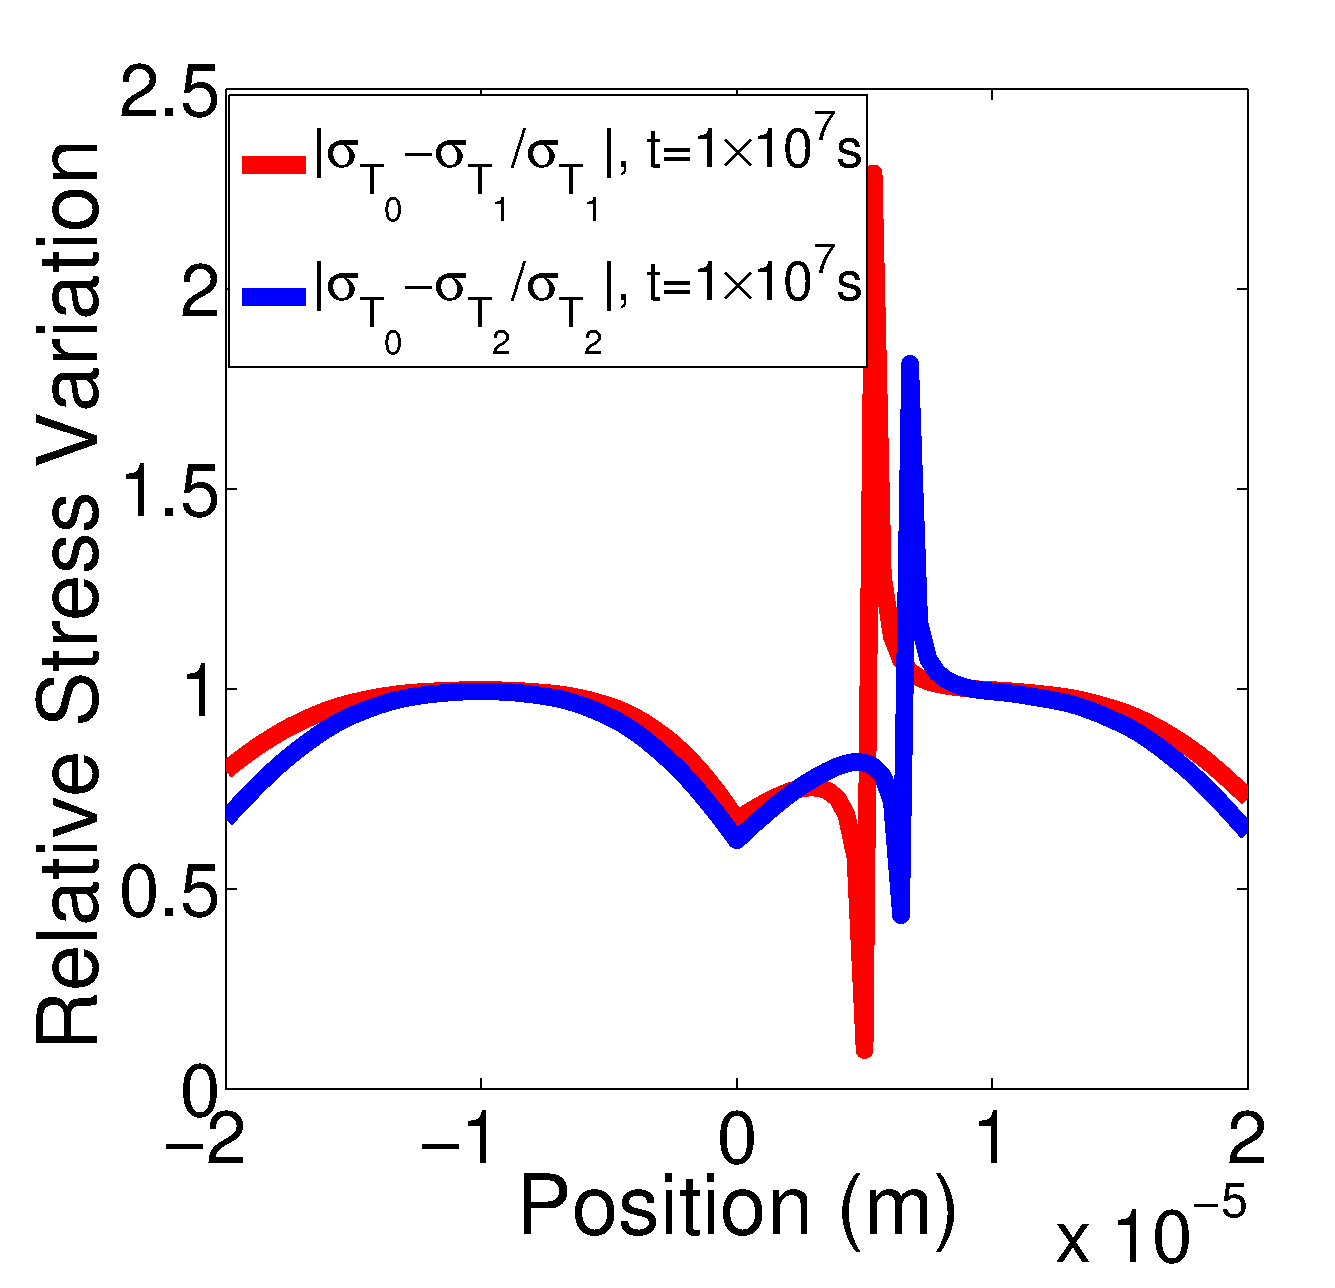
\includegraphics[width=0.45\columnwidth]{RelativeStress.eps}
% \label{fig:NTRStress}}
% \caption{The real results considering different temperature environment in COMSOL. (a) the stress evolution; (b) the relative stress variation.}
% \label{fig:NoteTemperature}
% \end{figure}

% n this work, for the first time, we propose an analytic method to
% calculate the stress evolution considering time-varying temperature
% effects during the void nucleation phase for some multi-branch
% interconnect trees, including the straight-line there-terminal wires,
% the T-shaped four-terminal wires and the cross-shaped five-terminal
% wires. The proposed closed-form expression can be used to calculate
% the hydrostatic stress evolution with time-varying temperature.


In this paper, we aim to resolve the mentioned problems for EM
model. We propose a new analytic expression hydrostatic stress
calculation for general multi-segment interconnect wire with multiple
terminals. The new method is based on the Laplace transformation
method on the Korhonen's equation with blocked atom flux boundary
conditions. The analytical solutions in terms of a set of auxiliary
basis functions using the complementary error function agree well with
the numerical analysis results. Our analysis further demonstrates that
using the first two dominant basis functions can lead to xx\% error,
which is sufficient for practical EM analysis.

The remainder of the paper is organized as follows. In Section
\ref{sec:reliability_modeling}, we induce the physics-based EM models
and analysis methods for the stress evolution during EM in simple
interconnect wires. Then we extend this analytic model to deal with a
general multi-segment interconnect wire case in Section
\ref{sec:multi_segment}. Experiment results and discussions for the
stress evolution modeling multi-segment (three-, five-, six-terminal)
interconnect wires are presented in Section
\ref{sec:experimental_results}. Concluding remarks are drawn in
Section \ref{sec:conclusion}.



